\documentclass[]{report}

\voffset=-1.5cm
\oddsidemargin=0.0cm
\textwidth = 480pt

\usepackage{framed}
\usepackage{subfiles}
\usepackage{graphics}
\usepackage{newlfont}
\usepackage{eurosym}
\usepackage{amsmath,amsthm,amsfonts}
\usepackage{amsmath}
\usepackage{color}
\usepackage{amssymb}
\usepackage{multicol}
\usepackage[dvipsnames]{xcolor}
\usepackage{graphicx}
\begin{document}
	%-------------------------------------------%
	
	\section{Regression Hypothesis Testing}
	\begin{itemize}
		\item To guard against making erroneous conclusions, a hypothesis test on the slope regression coefficient is
		recommended.
		\item The null hypothesis expresses the conservative viewpoint that no linear relationship between X and Y exists, and that the true value of the slope is zero.
		\item The alternative hypothesis is that there is a linear relationship between X and Y, and that the slope is not zero.
	\end{itemize}
	\begin{eqnarray}
	\mbox{H}_{0} : \beta_1 = 0 \\
	\mbox{H}_{1} : \beta_1 \neq 0 
	\end{eqnarray}
	Remember to describe the hypotheses in your answers.
	
	
	%-------------------------------------------%
	
	\subsection{Regression: Hypothesis Testing}
	\begin{itemize}
		\item The test statistic for this test follows the general form of all test statistics.
		\item The observed value is the slope estimate $b_1$ derived from the Least Squares estimation.
		\item The expected value under the null hypothesis is 0.
		\item The standard error is a complex two step calculation. (Formulae given in exam paper).
	\end{itemize}
	
	%-------------------------------------------%
	
	\subsection{Regression: Hypothesis Testing}
	\begin{figure}[h!]
		% Requires \usepackage{graphicx}
		\includegraphics[scale=0.7]{images/TestStat.jpg}\\
	\end{figure}
	
	%-------------------------------------------%
	
	\subsection{Regression: Hypothesis Testing}
	\begin{itemize}
		\item If the assumptions of the regression model are satisfied, this
		statistic has a Student t-distribution with n - 2 degrees of freedom.
		\item For large n this is approximately standard normal.
		\item The critical value for this test is $t_{(n-2,\alpha/2)}$
		\item (This is the same procedures as for the previous section, but with $n-2$ degrees of freedom, rather than $n-1$).
	\end{itemize}
	
	%-------------------------------------------%
	
	\subsection{Regression: Hypothesis Testing}
	Suppose that for some regression model, we have computed the following values
	\[ \hat{y} = 11.3 + 6.11 x\]
	
	\begin{multicols}{2}
	\begin{itemize}
		\item number of observations n=7,
		\item slope estimate $b_1$ = 6.11,
		\item $S_{XX}$ = 28,
		\item $S_{YY}$ = 1045.714.
		\item $S_{XY}$ = 171
	\end{itemize}
	\end{multicols}
	
	%-------------------------------------------%
	
	\subsection{Regression: Hypothesis Testing}
	\begin{figure}[h!]
		% Requires \usepackage{graphicx}
		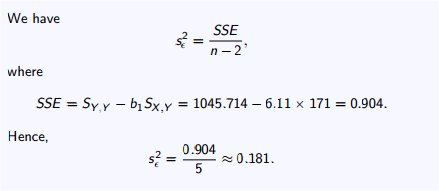
\includegraphics[scale=0.7]{images/TestStat2.jpg}\\
	\end{figure}
	
	%-------------------------------------------%
	
%	\subsection{Regression: Hypothesis Testing}
%	\begin{figure}
%		% Requires \usepackage{graphicx}
%		\includegraphics[scale=0.7]{images/TestStat3.jpg}\\
%	\end{figure}
	Test Statistic $TS = 76.375$
	
	%-------------------------------------------%
	
	\subsection{Regression: Hypothesis Testing}
	\begin{itemize}
		\item Two sided inference procedure, with significance level $\alpha=0.05$.
		\item Small sample size (n=7), degrees of freedom (n-2=5)
		\item The critical value is 2.571.
		\item Since $|TS|>CV$  we reject the null hypothesis. There is very strong evidence
		that variable Y changes with variable X.
	\end{itemize}
	
	%-------------------------------------------%
	
	\subsection{Regression: Hypothesis Testing}
	It should be noted that this test is not useful for detecting
	non-monotonic (i.e. certain non-linear) dependencies (for example,
	the quadratic like relationship plotted as one of the examples at
	the beginning of the chapter)
	
	%-------------------------------------------%
	SCHAUM OUTLINES
\newpage
		Part v: Hypothesis test on the slope.
		
		
		If the true value of the slope is zero, then there is no relationship between volume and pressure.
		
		(i.e. Null hypothesis means that Pressure doesnt depend on volume).
		
		
		The null and alternative hypotheses are as follows
		
		Ho:1= 0  	 The true value of the slope is zero
		
		
		The true value of the slope is not zero
		
		
		
		
		\begin{itemize}
			\item Let us assume a significance value of 5\% (0.05). Also, this hypothesis is a two tailed test. 
			
			\item If the p-value (referred to by SPSS as the "sig.") is greater than 0.025, we fail to reject the null hypothesis. We can not rightly contradict the statement that the true slope is zero.
			
			\item If the p-value is less than 0.025, we reject the null hypothesis.
			
			\item We reject the null hypothesis, accepting the alternative hypothesis that the true slope is not zero.
			
			\item (If the true slope is not zero, there two variable are not independent of each other).
			
			\item Here the p-value is very very low ("\texttt{sig}"  is 0.000). It is less than our threshold of 0.025. Therefore we reject the null hypothesis.
		\end{itemize}
	\section{Hypothesis Testing of Regression Estimates}

	\begin{itemize}
		\item We often require to test whether a slope estimate is zero.
		\item If the slope is zero, then there is no linear relationship between $X$ and $Y$.
	\end{itemize}
	
	%-------------------------------------------------%
	\noindent \textbf{Standard Error of Slope Estimate}
	\[S.E(b_1) = \sqrt{\frac{s^2}{S_{XX}}} \]
	
	\[s^2 = \frac{SSE}{n-2} \]
	\[SSE = S_{YY}- b_1S_{XY}\]

	$H_0: \beta_1 = 0$\\
	$H_1: \beta_1 \neq 0$\\
	
	
	\section{Hypothesis Testing of Regression Estimates}

	\begin{itemize}
		\item We often require to test whether a slope estimate is zero.
		\item If the slope is zero, then there is no linear relationship between $X$ and $Y$.
	\end{itemize}
	

	
	%-------------------------------------------------%
	
	\subsection{Hypothesis Testing of Regression Estimate}
	
	\begin{description}
		\item[$H_0$:] $\beta_1 = 0$  The True value of the slope is zero
		\item[$H_1:$] $\beta_1 \neq 0$ The True value of the slope is zero
	\end{description}

	\section{Inference for Regression}
	To determine the confidence interval for the slope we use the
	following equation:
	\begin{equation}
	b \pm t_{1-\alpha/2,n-2} S.E.(b)
	\end{equation}
	
	\begin{itemize}
		\item b = Estimation of Slope (0.0251643) \item S.E.(b) = Standard
		Error of Slope(0.0002656) \item n = Sample Size (7) \item $\alpha$
		= Alpha Value (5\%) \item $t_{1-\alpha/2,n-2}$ = Quantile Value
		from Student’s t-distribution (2.570582)
	\end{itemize}
	
	\begin{equation}
	(0.0251643) \pm ( 2.570582 \times 0.0002656) = [ 0.0245,0.0258 ]
	\end{equation}

\newpage


%--------------------------------------------------------------------%


\subsection{Significance Test of the Correlation Estimate}

%% {-1cm}
\textbf{Testing using Student's t-distribution}
%% {0.5cm}

For pairs from an uncorrelated bivariate normal distribution, the sampling distribution of Pearson's correlation coefficient follows Student's t-distribution with degrees of freedom n - 2. 




Specifically, if the underlying variables have a bivariate normal distribution, the variable
\[ t_{TS} = r\sqrt{\frac{n-2}{1 - r^2}} \]



\begin{itemize}
	\item Test statistic follows follows Student's t-distribution with degrees of freedom n - 2.
	\item Compare the test statistic to quantile with $n-2$ degrees of freedom for specified confidence level.
\end{itemize}


%--------------------------------------------------------------------%

%--------------------------------------------------------------------%

\subsection{Significance Test of the Correlation Estimate}

%% {-0.50cm}
\textbf{Example }

\begin{itemize}
	\item Sample Size : $n = 11$
	\item Correlation Coefficient : $r = 0.922$
\end{itemize}
%% {0.2cm}

The Test Statistic $t_{TS}$ is computed as follows:\\
\[ t_{TS} \; = \; r\sqrt{\frac{n-2}{1 - r^2}} \; = \; 0.922 \sqrt{\frac{11-2}{1 - 0.85}}  \]
%% {0.2cm}
\[ t_{TS} = 0.922 \sqrt{\frac{9}{0.15}} \; = \;  7.1417 \]





\begin{center}
	\begin{tabular}{|c||c|c|c|c|}
		\hline dfs ($\nu$) &  & $0.025$ & $0.05$ &  \\ \hline
		\hline $\ldots$ &  & $\ldots$ & $\ldots$ &  \\ 
		\hline 8 & $\ldots$ &  & $\ldots$  &  $\ldots$ \\ 
		\hline 9 & $\ldots$ &  & 2.262  &  $\ldots$ \\ 
		\hline 10 & $\ldots$ & & 2.228   & $\ldots$ \\ 
		\hline 11 & $\ldots$ & & 2.201    & $\ldots$ \\ 
		\hline 12 & $\ldots$ & & 2.179   & $\ldots$ \\ 
		\hline \phantom{spaces} & \phantom{spaces} & \phantom{spaces}  & \phantom{spaces} & \phantom{spaces} \\ 
		\hline 
	\end{tabular} 
\end{center}
\begin{itemize}
	\item[df] : degrees of freedom
\end{itemize}


%-------------------------------------------------%

\begin{itemize}
	\item Let us assume a significance value of 5\% (0.05). Also, this hypothesis is a two tailed test. 
	
	\item If the p-value (referred to by SPSS as the "sig.") is greater than 0.025, we fail to reject the null hypothesis. We can not rightly contradict the statement that the true slope is zero.
	
	\item If the p-value is less than 0.025, we reject the null hypothesis.
	
	\item We reject the null hypothesis, accepting the alternative hypothesis that the true slope is not zero.
	
	\item (If the true slope is not zero, there two variable are not independent of each other).
	
	\item Here the p-value is very very low ("\texttt{sig}"  is 0.000). It is less than our threshold of 0.025. Therefore we reject the null hypothesis.
\end{itemize}





\subsection{Random Samples}
\begin{itemize}
	\item Consider two random samples drawn from X and Y respectively.
	\item When these observations are plotted on a scatterplot, it
	may be the case that some sort of relationship \textbf{appears} to exist (when in fact it doesn't).
	\item The smaller the number of observations, the more likely this erroneous conclusion will occur.
\end{itemize}




%-------------------------------------------%

\subsection{Regression: Hypothesis Testing}
%\begin{figure}
%% Requires \usepackage{graphicx}
%\includegraphics[scale=0.7]{TestStat.jpg}\\
%\end{figure}
%
%-------------------------------------------%

\subsection{Regression: Hypothesis Testing}
\begin{itemize}
	\item If the assumptions of the regression model are satisfied, this
	statistic has a Student t-distribution with n - 2 degrees of freedom.
	\item For large n this is approximately standard normal.
	\item The critical value for this test is $t_{(n-2,\alpha/2)}$
	\item This is the same procedures as for the previous section, but with $n-2$ degrees of freedom, rather than $n-1$).
\end{itemize}



%-------------------------------------------%

\textbf{Regression: Hypothesis Testing}
\begin{figure}
	% Requires \usepackage{graphicx}
	\includegraphics[scale=0.7]{images/TestStat.jpg}\\
\end{figure}

%
%\textbf{Regression: Hypothesis Testing}
%\begin{figure}
%  % Requires \usepackage{graphicx}
%  \includegraphics[scale=0.7]{images/TestStat.jpg}\\
%\end{figure}
%
%-------------------------------------------%



\subsection{Regression: Hypothesis Testing}
Suppose that for some regression model, we have computed the following values
\[ \hat{y} = 11.3 + 6.11 x\]
\begin{itemize}
	\item number of observations n=7,
	\item slope estimate $b_1$ = 6.11,
	\item $S_{XX}$ = 28,
	\item $S_{YY}$ = 1045.714.
	\item $S_{XY}$ = 171
\end{itemize}

%-------------------------------------------%

%-------------------------------------------%
\subsection{Regression: Hypothesis Testing}
\begin{itemize}
	\item Two sided inference procedure, with significance level $\alpha=0.05$.
	\item Small sample size (n=7), degrees of freedom (n-2=5)
	\item The critical value is 2.571.
	\item Since $|TS|>CV$  our conlusion is that we reject the null hypothesis. There is very strong evidence
	that variable Y changes with variable X.
\end{itemize}



%-------------------------------------------%

\subsection{Regression: Hypothesis Testing}
It should be noted that this test is not useful for detecting
non-monotonic (i.e. certain non-linear) dependencies (for example,
the quadratic like relationship plotted as one of the examples at
the beginning of the chapter)					



\bigskip

\section{Inference for Regression}
To determine the confidence interval for the slope we use the
following equation:
\begin{equation}
b \pm t_{1-\alpha/2,n-2} S.E.(b)
\end{equation}

\begin{itemize}
	\item b = Estimation of Slope (0.0251643) \item S.E.(b) = Standard
	Error of Slope(0.0002656) \item n = Sample Size (7) \item $\alpha$
	= Alpha Value (5\%) \item $t_{1-\alpha/2,n-2}$ = Quantile Value
	from Student’s t-distribution (2.570582)
\end{itemize}

\begin{equation}
(0.0251643) \pm ( 2.570582 \times 0.0002656) = [ 0.0245,0.0258 ]
\end{equation}


\subsection{Regression example}

In a medical experiment concerning 12 patients with a certain type of ear condition,
the following measurements were made for blood flow (y) and auricular pressure (x):

\begin{verbatim}
x<-c(8.5, 9.8, 10.8, 11.5, 11.2, 9.6, 10.1, 13.5, 14.2, 11.8, 8.7, 6.8)
y<-c(3 ,12, 10, 14, 8 ,7 ,9 ,13, 17, 10, 5 ,5)
\end{verbatim}


($S_x =126.5 S_{xx} =1,381.85 S_y =113 S_{yy} =1251, S_{xy} =1272.2$)


\begin{itemize}
	\item Calculate the equation of the least-squares fitted regression line of blood flow
	on auricular pressure.
	\item Confirm the following values: Sx =126.5, Sxx =1381.85, Sy =113, Syy =1251, Sxy =1272.2.
	\item Calculate the correlation coefficient.
	
	\begin{verbatim}
	> cor(x,y)
	[1] 0.8521414
	\end{verbatim}
\end{itemize}



\subsection{Standard Error of Slope Estimate}
\[S.E(b_1) = \sqrt{\frac{s^2}{S_{XX}}} \]

\[s^2 = \frac{SSE}{n-2} \]
\[SSE = S_{YY}- b_1S_{XY}\]


%-------------------------------------------------%

\subsection{Hypothesis Testing of Regression Estimate}

\begin{description}
	\item[$H_0$:] $\beta_1 = 0$  The True value of the slope is zero
	\item[$H_1:$] $\beta_1 \neq 0$ The True value of the slope is zero
\end{description}


$H_0: \beta_1 = 0$\\
$H_1: \beta_1 \neq 0$\\


	
\end{document}
